%% bare_jrnl.tex
%% V1.4b
%% 2015/08/26
%% by Michael Shell
%% see http://www.michaelshell/
%% for current contact information.
%% 
%% This is a skeleton file demonstrating the use of IEEEtran.cls
%% (requires IEEEtran.cls version 1.8b or later) with an IEEE
%% journal paper.
%%
%% Support sites:
%% http://www.michaelshell.org/tex/ie eetran/
%% http://www.ctan.org/pkg/ieeetran
%% and 
%% http://www.ieee.org/

%%*************************************************************************
%% Legal Notice:
%% This code is offered as-is without any warranty either expressed or
%% implied; without even the implied warranty of MERCHANTABILITY or
%% FITNESS FOR A PARTICULAR PURPOSE! 
%% User assumes all risk.
%% In no event shall the IEEE or any contributor to this code be liable for
%% any damages or losses, including, but not limited to, incidental,
%% consequential, or any other damages, resulting from the use or misuse
%% of any information contained here.
%%
%% All comments are the opinions of their respective authors and are not
%% necessarily endorsed by the IEEE.
%%
%% This work is distributed under the LaTeX Project Public License (LPPL)
%% ( http://www.latex-project.org/ ) version 1.3, and may be freely used,
%% distributed and modified. A copy of the LPPL, version 1.3, is included
%% in the base LaTeX documentation of all distributions of LaTeX released
%% 2003/12/01 or later.
%% Retain all contribution notices and credits.
%% ** Modified files should be clearly indicated as such, including  **
%% ** renaming them and changing author support contact information. **
%%*************************************************************************


% *** Authors should verify (and, if needed, correct) their LaTeX system  ***
% *** with the testflow diagnostic prior to trusting their LaTeX platform ***
% *** with production work. The IEEE's font choices and paper sizes can   ***
% *** trigger bugs that do not appear when using other class files.       ***                          ***
% The testflow support page is at:
% http://www.michaelshell.org/tex/testflow/



\documentclass[journal]{IEEEtran}

%
% If IEEEtran.cls has not been installed into the LaTeX system files,
% manually specify the path to it like:
% \documentclass[journal]{../sty/IEEEtran}





% Some very useful LaTeX packages include:
% (uncomment the ones you want to load)


% *** MISC UTILITY PACKAGES ***
%
%\usepackage{ifpdf}
% Heiko Oberdiek's ifpdf.sty is very useful if you need conditional
% compilation based on whether the output is pdf or dvi.
% usage:
% \ifpdf
%   % pdf code
% \else
%   % dvi code
% \fi
% The latest version of ifpdf.sty can be obtained from:
% http://www.ctan.org/pkg/ifpdf
% Also, note that IEEEtran.cls V1.7 and later provides a builtin
% \ifCLASSINFOpdf conditional that works the same way.
% When switching from latex to pdflatex and vice-versa, the compiler may
% have to be run twice to clear warning/error messages.






% *** CITATION PACKAGES ***
%
\usepackage{cite}
% cite.sty was written by Donald Arseneau
% V1.6 and later of IEEEtran pre-defines the format of the cite.sty package
% \cite{} output to follow that of the IEEE. Loading the cite package will
% result in citation numbers being automatically sorted and properly
% "compressed/ranged". e.g., [1], [9], [2], [7], [5], [6] without using
% cite.sty will become [1], [2], [5]--[7], [9] using cite.sty. cite.sty's
% \cite will automatically add leading space, if needed. Use cite.sty's
% noadjust option (cite.sty V3.8 and later) if you want to turn this off
% such as if a citation ever needs to be enclosed in parenthesis.
% cite.sty is already installed on most LaTeX systems. Be sure and use
% version 5.0 (2009-03-20) and later if using hyperref.sty.
% The latest version can be obtained at:
% http://www.ctan.org/pkg/cite
% The documentation is contained in the cite.sty file itself.






% *** GRAPHICS RELATED PACKAGES ***
%
\ifCLASSINFOpdf
  \usepackage[pdftex]{graphicx}
  % declare the path(s) where your graphic files are
  % \graphicspath{{../pdf/}{../jpeg/}}
  % and their extensions so you won't have to specify these with
  % every instance of \includegraphics
  % \DeclareGraphicsExtensions{.pdf,.jpeg,.png}
\else
  % or other class option (dvipsone, dvipdf, if not using dvips). graphicx
  % will default to the driver specified in the system graphics.cfg if no
  % driver is specified.
  % \usepackage[dvips]{graphicx}
  % declare the path(s) where your graphic files are
  % \graphicspath{{../eps/}}
  % and their extensions so you won't have to specify these with
  % every instance of \includegraphics
  % \DeclareGraphicsExtensions{.eps}
\fi
% graphicx was written by David Carlisle and Sebastian Rahtz. It is
% required if you want graphics, photos, etc. graphicx.sty is already
% installed on most LaTeX systems. The latest version and documentation
% can be obtained at: 
% http://www.ctan.org/pkg/graphicx
% Another good source of documentation is "Using Imported Graphics in
% LaTeX2e" by Keith Reckdahl which can be found at:
% http://www.ctan.org/pkg/epslatex
%
% latex, and pdflatex in dvi mode, support graphics in encapsulated
% postscript (.eps) format. pdflatex in pdf mode supports graphics
% in .pdf, .jpeg, .png and .mps (metapost) formats. Users should ensure
% that all non-photo figures use a vector format (.eps, .pdf, .mps) and
% not a bitmapped formats (.jpeg, .png). The IEEE frowns on bitmapped formats
% which can result in "jaggedy"/blurry rendering of lines and letters as
% well as large increases in file sizes.
%
% You can find documentation about the pdfTeX application at:
% http://www.tug.org/applications/pdftex





% *** MATH PACKAGES ***
%
\usepackage{amsmath}
% A popular package from the American Mathematical Society that provides
% many useful and powerful commands for dealing with mathematics.
%
% Note that the amsmath package sets \interdisplaylinepenalty to 10000
% thus preventing page breaks from occurring within multiline equations. Use:
\interdisplaylinepenalty=2500
% after loading amsmath to restore such page breaks as IEEEtran.cls normally
% does. amsmath.sty is already installed on most LaTeX systems. The latest
% version and documentation can be obtained at:
% http://www.ctan.org/pkg/amsmath





% *** SPECIALIZED LIST PACKAGES ***
%
%\usepackage{algorithmic}
% algorithmic.sty was written by Peter Williams and Rogerio Brito.
% This package provides an algorithmic environment fo describing algorithms.
% You can use the algorithmic environment in-text or within a figure
% environment to provide for a floating algorithm. Do NOT use the algorithm
% floating environment provided by algorithm.sty (by the same authors) or
% algorithm2e.sty (by Christophe Fiorio) as the IEEE does not use dedicated
% algorithm float types and packages that provide these will not provide
% correct IEEE style captions. The latest version and documentation of
% algorithmic.sty can be obtained at:
% http://www.ctan.org/pkg/algorithms
% Also of interest may be the (relatively newer and more customizable)
% algorithmicx.sty package by Szasz Janos:
% http://www.ctan.org/pkg/algorithmicx




% *** ALIGNMENT PACKAGES ***
%
\usepackage{array}
% Frank Mittelbach's and David Carlisle's array.sty patches and improves
% the standard LaTeX2e array and tabular environments to provide better
% appearance and additional user controls. As the default LaTeX2e table
% generation code is lacking to the point of almost being broken with
% respect to the quality of the end results, all users are strongly
% advised to use an enhanced (at the very least that provided by array.sty)
% set of table tools. array.sty is already installed on most systems. The
% latest version and documentation can be obtained at:
% http://www.ctan.org/pkg/array


% IEEEtran contains the IEEEeqnarray family of commands that can be used to
% generate multiline equations as well as matrices, tables, etc., of high
% quality.




% *** SUBFIGURE PACKAGES ***
\ifCLASSOPTIONcompsoc
  \usepackage[caption=false,font=normalsize,labelfont=sf,textfont=sf]{subfig}
\else
\usepackage[caption=false,font=footnotesize]{subfig}
\fi
% subfig.sty, written by Steven Douglas Cochran, is the modern replacement
% for subfigure.sty, the latter of which is no longer maintained and is
% incompatible with some LaTeX packages including fixltx2e. However,
% subfig.sty requires and automatically loads Axel Sommerfeldt's caption.sty
% which will override IEEEtran.cls' handling of captions and this will result
% in non-IEEE style figure/table captions. To prevent this problem, be sure
% and invoke subfig.sty's "caption=false" package option (available since
% subfig.sty version 1.3, 2005/06/28) as this is will preserve IEEEtran.cls
% handling of captions.
% Note that the Computer Society format requires a larger sans serif font
% than the serif footnote size font used in traditional IEEE formatting
% and thus the need to invoke different subfig.sty package options depending
% on whether compsoc mode has been enabled.
%
% The latest version and documentation of subfig.sty can be obtained at:
% http://www.ctan.org/pkg/subfig




% *** FLOAT PACKAGES ***
%
%\usepackage{fixltx2e}
% fixltx2e, the successor to the earlier fix2col.sty, was written by
% Frank Mittelbach and David Carlisle. This package corrects a few problems
% in the LaTeX2e kernel, the most notable of which is that in current
% LaTeX2e releases, the ordering of single and double column floats is not
% guaranteed to be preserved. Thus, an unpatched LaTeX2e can allow a
% single column figure to be placed prior to an earlier double column
% figure.
% Be aware that LaTeX2e kernels dated 2015 and later have fixltx2e.sty's
% corrections already built into the system in which case a warning will
% be issued if an attempt is made to load fixltx2e.sty as it is no longer
% needed.
% The latest version and documentation can be found at:
% http://www.ctan.org/pkg/fixltx2e


%\usepackage{stfloats}
% stfloats.sty was written by Sigitas Tolusis. This package gives LaTeX2e
% the ability to do double column floats at the bottom of the page as well
% as the top. (e.g., "\begin{figure*}[!b]" is not normally possible in
% LaTeX2e). It also provides a command:
%\fnbelowfloat
% to enable the placement of footnotes below bottom floats (the standard
% LaTeX2e kernel puts them above bottom floats). This is an invasive package
% which rewrites many portions of the LaTeX2e float routines. It may not work
% with other packages that modify the LaTeX2e float routines. The latest
% version and documentation can be obtained at:
% http://www.ctan.org/pkg/stfloats
% Do not use the stfloats baselinefloat ability as the IEEE does not allow
% \baselineskip to stretch. Authors submitting work to the IEEE should note
% that the IEEE rarely uses double column equations and that authors should try
% to avoid such use. Do not be tempted to use the cuted.sty or midfloat.sty
% packages (also by Sigitas Tolusis) as the IEEE does not format its papers in
% such ways.
% Do not attempt to use stfloats with fixltx2e as they are incompatible.
% Instead, use Morten Hogholm'a dblfloatfix which combines the features
% of both fixltx2e and stfloats:
%
% \usepackage{dblfloatfix}
% The latest version can be found at:
% http://www.ctan.org/pkg/dblfloatfix




%\ifCLASSOPTIONcaptionsoff
%  \usepackage[nomarkers]{endfloat}
% \let\MYoriglatexcaption\caption
% \renewcommand{\caption}[2][\relax]{\MYoriglatexcaption[#2]{#2}}
%\fi
% endfloat.sty was written by James Darrell McCauley, Jeff Goldberg and 
% Axel Sommerfeldt. This package may be useful when used in conjunction with 
% IEEEtran.cls'  captionsoff option. Some IEEE journals/societies require that
% submissions have lists of figures/tables at the end of the paper and that
% figures/tables without any captions are placed on a page by themselves at
% the end of the document. If needed, the draftcls IEEEtran class option or
% \CLASSINPUTbaselinestretch interface can be used to increase the line
% spacing as well. Be sure and use the nomarkers option of endfloat to
% prevent endfloat from "marking" where the figures would have been placed
% in the text. The two hack lines of code above are a slight modification of
% that suggested by in the endfloat docs (section 8.4.1) to ensure that
% the full captions always appear in the list of figures/tables - even if
% the user used the short optional argument of \caption[]{}.
% IEEE papers do not typically make use of \caption[]'s optional argument,
% so this should not be an issue. A similar trick can be used to disable
% captions of packages such as subfig.sty that lack options to turn off
% the subcaptions:
% For subfig.sty:
% \let\MYorigsubfloat\subfloat
% \renewcommand{\subfloat}[2][\relax]{\MYorigsubfloat[]{#2}}
% However, the above trick will not work if both optional arguments of
% the \subfloat command are used. Furthermore, there needs to be a
% description of each subfigure *somewhere* and endfloat does not add
% subfigure captions to its list of figures. Thus, the best approach is to
% avoid the use of subfigure captions (many IEEE journals avoid them anyway)
% and instead reference/explain all the subfigures within the main caption.
% The latest version of endfloat.sty and its documentation can obtained at:
% http://www.ctan.org/pkg/endfloat
%
% The IEEEtran \ifCLASSOPTIONcaptionsoff conditional can also be used
% later in the document, say, to conditionally put the References on a 
% page by themselves.




% *** PDF, URL AND HYPERLINK PACKAGES ***
%
\usepackage{url}
% url.sty was written by Donald Arseneau. It provides better support for
% handling and breaking URLs. url.sty is already installed on most LaTeX
% systems. The latest version and documentation can be obtained at:
% http://www.ctan.org/pkg/url
% Basically, \url{my_url_here}.




% *** Do not adjust lengths that control margins, column widths, etc. ***
% *** Do not use packages that alter fonts (such as pslatex).         ***
% There should be no need to do such things with IEEEtran.cls V1.6 and later.
% (Unless specifically asked to do so by the journal or conference you plan
% to submit to, of course. )


%%%%%%%%%%%%%%%%%%%%%%%%%%% AUTHOR'S HEADER %%%%%%%%%%%%%%%%%%%%%%%%%%%%%%%%
\usepackage{xspace}
\newcommand*{\eg}{e.g.\@\xspace}
\newcommand*{\ie}{i.e.\@\xspace}
\newcommand*{\resp}{resp.\@\xspace}
\newcommand*{\vs}{vs.\@\xspace}
\newcommand\Fscore{$F_1$-score}

\usepackage{mathptmx}
\usepackage{amsmath}
\usepackage{amssymb}
\usepackage{amsthm}
\newtheorem{thm}{Theorem}[section]
\newtheorem{lem}[thm]{Lemma}
\newtheorem{prop}[thm]{Proposition}
\newtheorem*{prop*}{Proposition}
\theoremstyle{remark}
\newtheorem*{remark}{Remark}
\renewcommand{\qedsymbol}{$\blacksquare$}
\usepackage{siunitx}
\usepackage{enumitem}
\usepackage{adjustbox}
\usepackage{stackengine}
\usepackage{url}
\urlstyle{same}
\usepackage{microtype}

\usepackage{xr}
\externaldocument{lostanlen2018spl}

% correct bad hyphenation here
\hyphenation{op-tical net-works semi-conduc-tor}

\begin{document}
%
% paper title
% Titles are generally capitalized except for words such as a, an, and, as,
% at, but, by, for, in, nor, of, on, or, the, to and up, which are usually
% not capitalized unless they are the first or last word of the title.
% Linebreaks \\ can be used within to get better formatting as desired.
% Do not put math or special symbols in the title.
%\title{Per-Channel Energy Normalization: Why and How}
%
%
% author names and IEEE memberships
% note positions of commas and nonbreaking spaces ( ~ ) LaTeX will not break
% a structure at a ~ so this keeps an author's name from being broken across
% two lines.
% use \thanks{} to gain access to the first footnote area
% a separate \thanks must be used for each paragraph as LaTeX2e's \thanks
% was not built to handle multiple paragraphs
%

%\author{Michael~Shell,~\IEEEmembership{Member,~IEEE,}
%        John~Doe,~\IEEEmembership{Fellow,~OSA,}
%        and~Jane~Doe,~\IEEEmembership{Life~Fellow,~IEEE}% <-this % stops a space
%\thanks{M. Shell was with the Department
%of Electrical and Computer Engineering, Georgia Institute of Technology, Atlanta,
%GA, 30332 USA e-mail: (see http://www.michaelshell.org/contact.html).}% <-this % stops a space
%\thanks{J. Doe and J. Doe are with Anonymous University.}% <-this % stops a space
%\thanks{Manuscript received April 19, 2005; revised August 26, 2015.}}

%\author{Vincent~Lostanlen, Justin~Salamon, Mark~Cartwright, Brian~McFee,\\
%Andrew~Farnsworth, Steve~Kelling, and Juan~Pablo~Bello% <-this % stops a space
%\thanks{V. Lostanlen, A. Farnsworth, and S. Kelling are with the Cornell Lab of Ornithology.
%J. Salamon, M. Cartwright, B. McFee, and J. P. Bello are with New York University.}% <-this % stops a space
%}

% note the % following the last \IEEEmembership and also \thanks - 
% these prevent an unwanted space from occurring between the last author name
% and the end of the author line. i.e., if you had this:
% 
% \author{....lastname \thanks{...} \thanks{...} }
%                     ^------------^------------^----Do not want these spaces!
%
% a space would be appended to the last name and could cause every name on that
% line to be shifted left slightly. This is one of those "LaTeX things". For
% instance, "\textbf{A} \textbf{B}" will typeset as "A B" not "AB". To get
% "AB" then you have to do: "\textbf{A}\textbf{B}"
% \thanks is no different in this regard, so shield the last } of each \thanks
% that ends a line with a % and do not let a space in before the next \thanks.
% Spaces after \IEEEmembership other than the last one are OK (and needed) as
% you are supposed to have spaces between the names. For what it is worth,
% this is a minor point as most people would not even notice if the said evil
% space somehow managed to creep in.



% The paper headers
\markboth{IEEE Signal Processing Letters,~Vol.~X, No.~Y, Submitted~July~2018, Revised~October~2018}%
{Lostanlen \MakeLowercase{\textit{et al.}}: \title{}}
% The only time the second header will appear is for the odd numbered pages
% after the title page when using the twoside option.
% 
% *** Note that you probably will NOT want to include the author's ***
% *** name in the headers of peer review papers.                   ***
% You can use \ifCLASSOPTIONpeerreview for conditional compilation here if
% you desire.




% If you want to put a publisher's ID mark on the page you can do it like
% this:
%\IEEEpubid{0000--0000/00\$00.00~\copyright~2015 IEEE}
% Remember, if you use this you must call \IEEEpubidadjcol in the second
% column for its text to clear the IEEEpubid mark.



% use for special paper notices
%\IEEEspecialpapernotice{(Invited Paper)}




% make the title area
%\maketitle

% Note that keywords are not normally used for peerreview papers.
%\begin{IEEEkeywords}
%Acoustic noise, acoustic sensors, acoustic signal detection, signal classification, spectrogram.
%\end{IEEEkeywords}

% For peer review papers, you can put extra information on the cover
% page as needed:
% \ifCLASSOPTIONpeerreview
% \begin{center} \bfseries EDICS Category: 3-BBND \end{center}
% \fi
%
% For peerreview papers, this IEEEtran command inserts a page break and
% creates the second title. It will be ignored for other modes.
\IEEEpeerreviewmaketitle


%%%%%%%%%%%%%%%%%%%%%%%%%%%%%%%%%%%%%%%%%%%%%%%%%%%%%%%%%%%%%%%%%%%%%%%%%%%%%%%%
%%%%%%%%%%%%%%%%%%%%%%%%% SUPPLEMENTARY MATERIAL %%%%%%%%%%%%%%%%%%%%%%%%%%%%%%%


\section*{Supplementary material}


\renewenvironment{proof}{}{\qed}

%\subsection{Extension of Figures \ref{fig:gaussianization}}

% \begin{figure}
% \centering
% \subfloat[Logarithmic transformation.]{%
% \stackunder{SONYC}{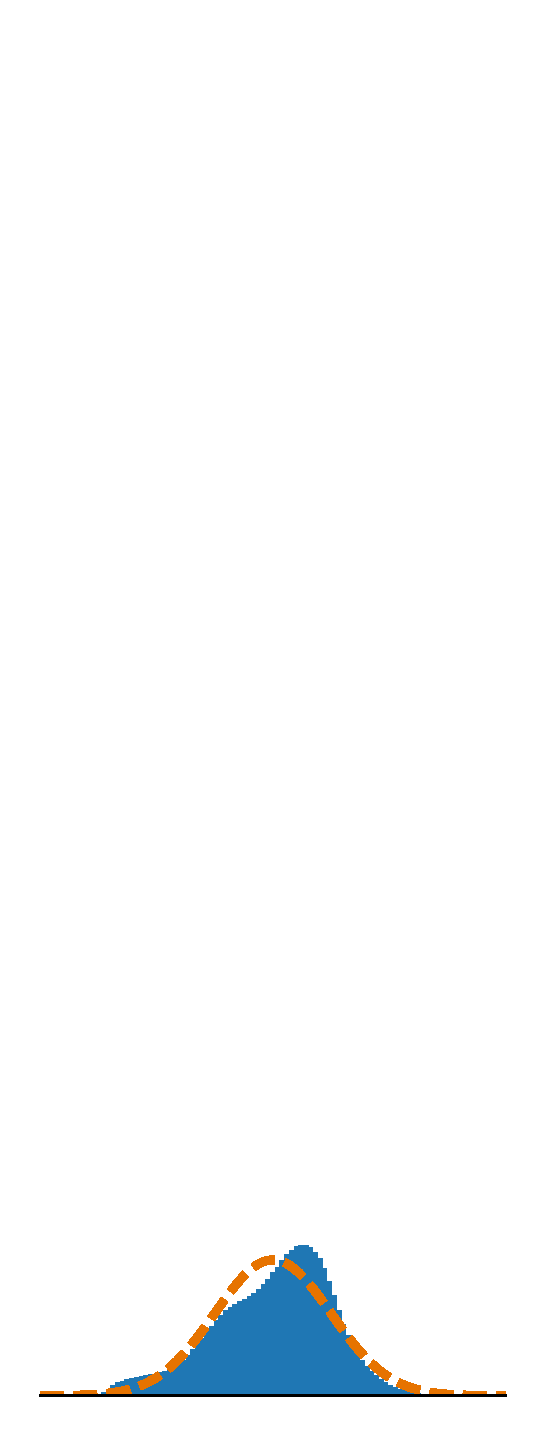
\includegraphics[width=0.33\linewidth,trim={0 0 0 20.5cm},clip]{SONYC-pcen_logE_histogram.eps}}
% \stackunder{DCASE 2013}{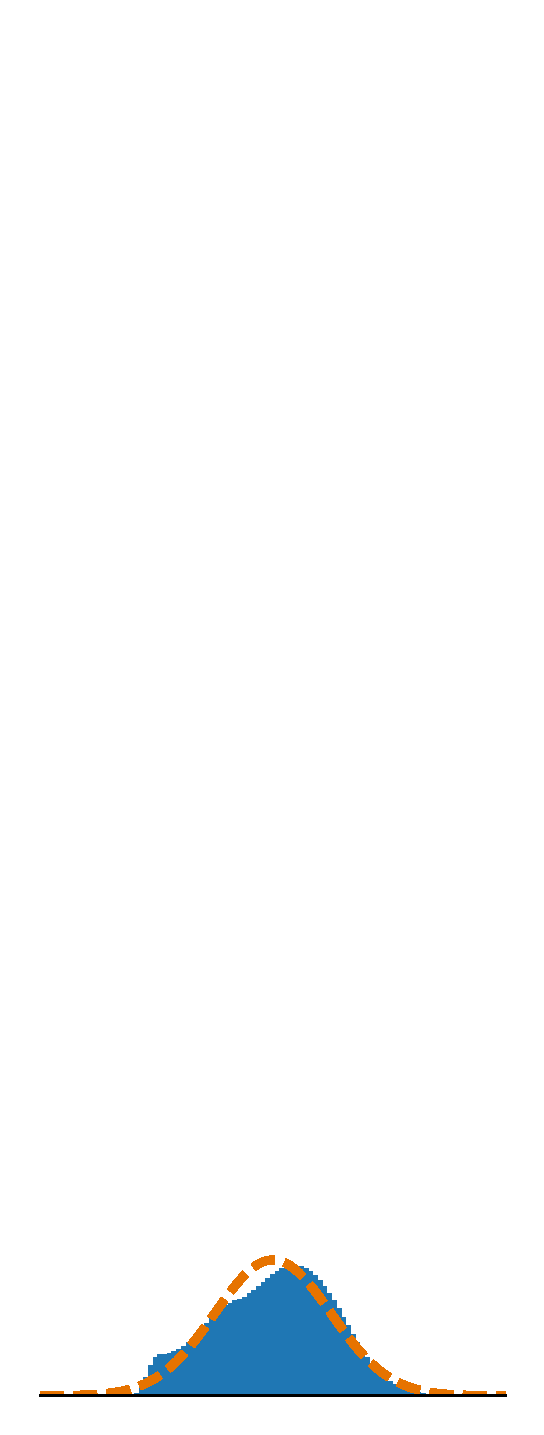
\includegraphics[width=0.33\linewidth,trim={0 0 0 20.5cm},clip]{DCASE2013-pcen_logE_histogram.eps}}
% \stackunder{BirdVox}{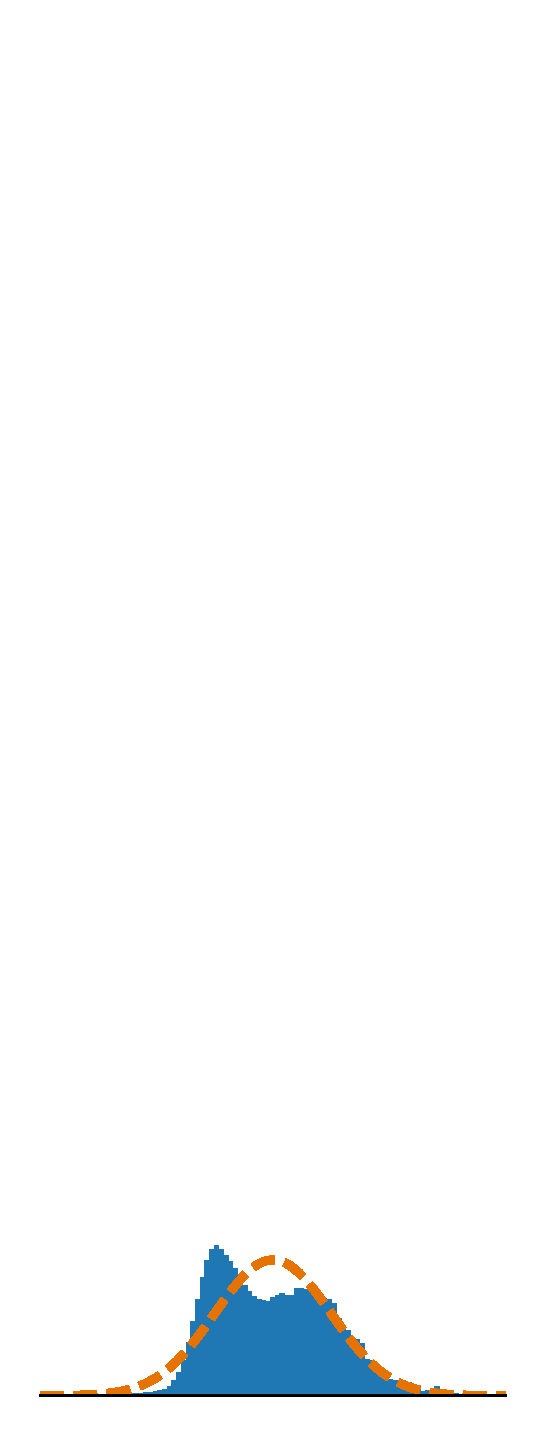
\includegraphics[width=0.33\linewidth,trim={0 0 0 20.5cm},clip]{BirdVox-pcen_logE_histogram.eps}}}
% \\
% \subfloat[Simple renormalization: $\mathbf{E} \mapsto \dfrac{\mathbf{E}}{\mathbf{E}\ast\boldsymbol{\phi}}$.]{%
% 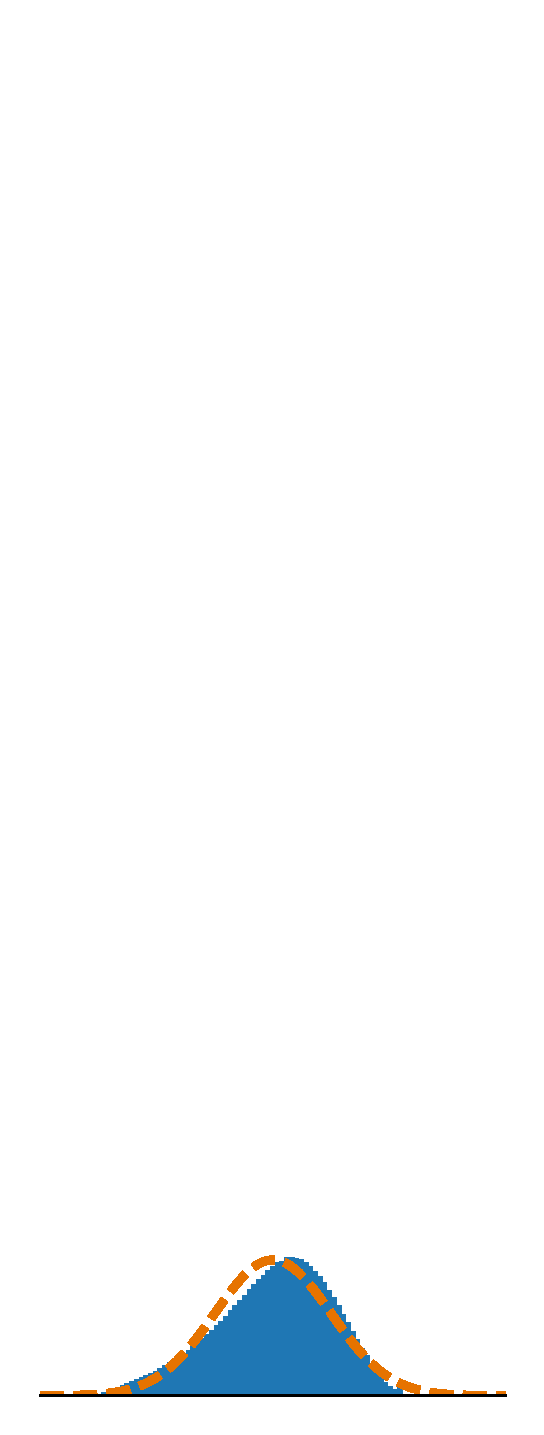
\includegraphics[width=0.33\linewidth,trim={0 0 0 20cm},clip]{SONYC-pcen_EoverM_histogram.eps}
% 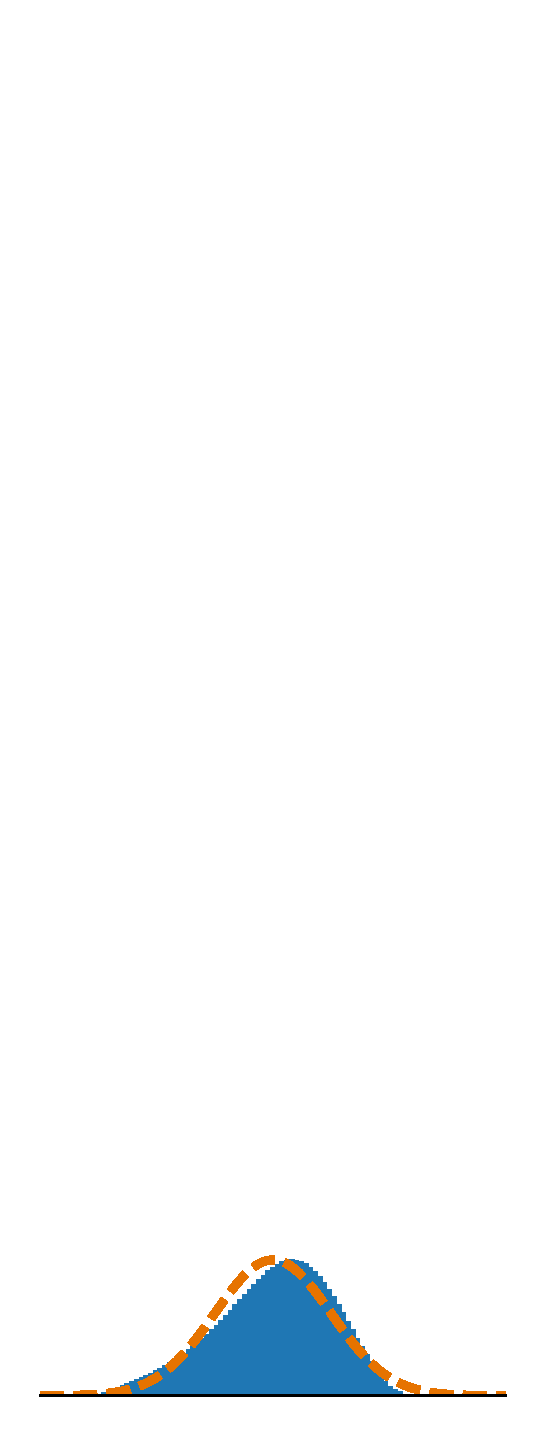
\includegraphics[width=0.33\linewidth,trim={0 0 0 20cm},clip]{DCASE2013-pcen_EoverM_histogram.eps}
% 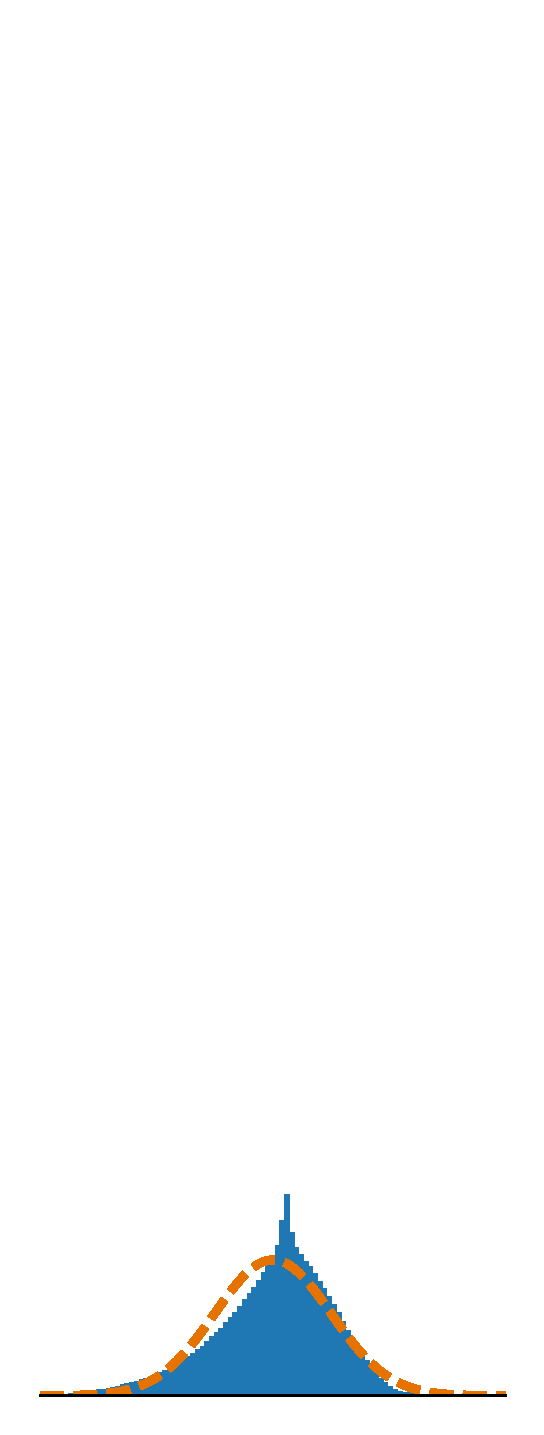
\includegraphics[width=0.33\linewidth,trim={0 0 0 20cm},clip]{BirdVox-pcen_EoverM_histogram.eps}}
% \\
% \subfloat[Renormalization with soft threshold: $\mathbf{E} \mapsto \dfrac{\mathbf{E}}{\varepsilon+(\mathbf{E}\ast\boldsymbol{\phi})}$.]{%
% 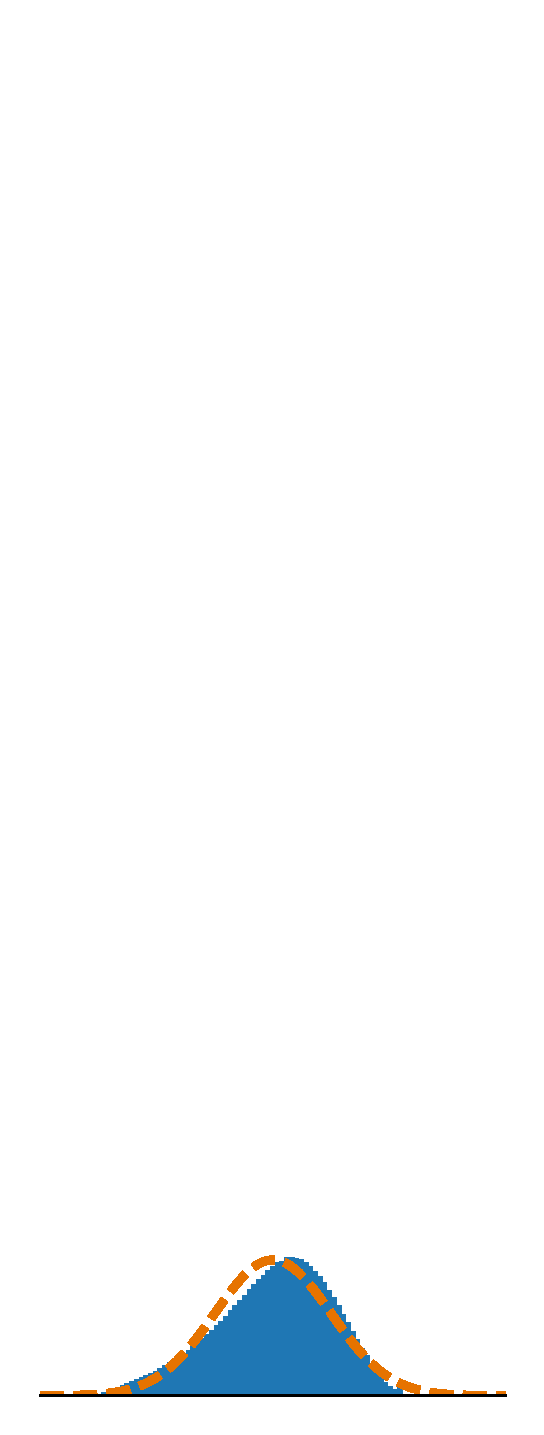
\includegraphics[width=0.33\linewidth,trim={0 0 0 20cm},clip]{SONYC-pcen_EoverMplusEps_histogram.eps}
% 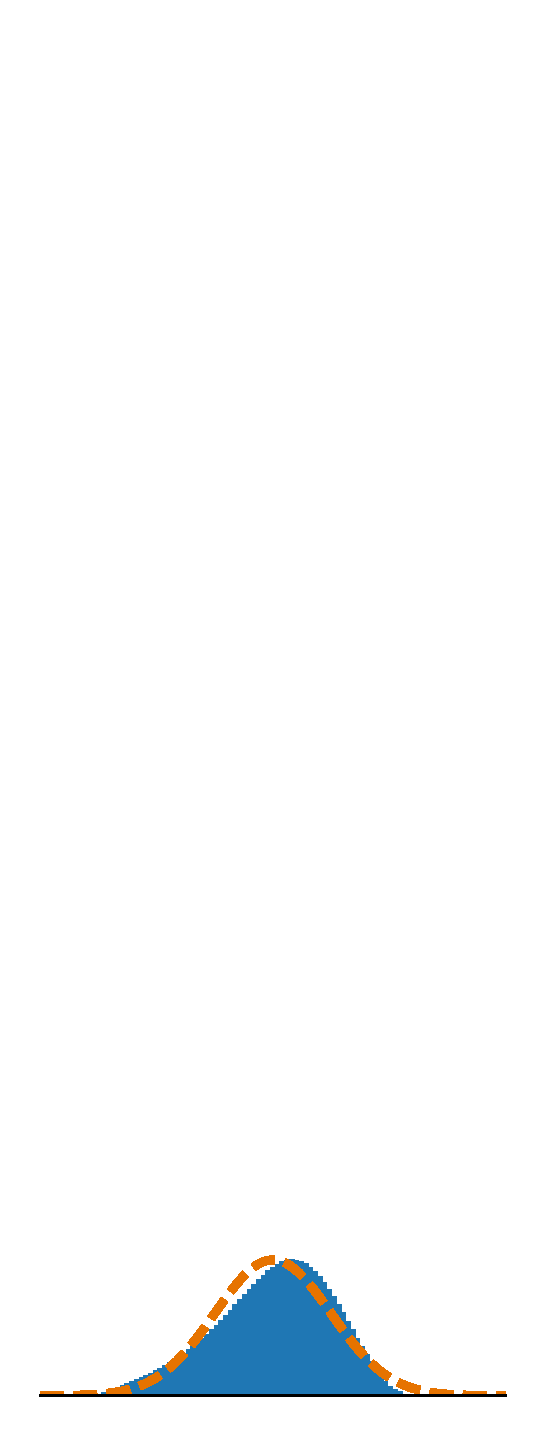
\includegraphics[width=0.33\linewidth,trim={0 0 0 20cm},clip]{DCASE2013-pcen_EoverMplusEps_histogram.eps}
% 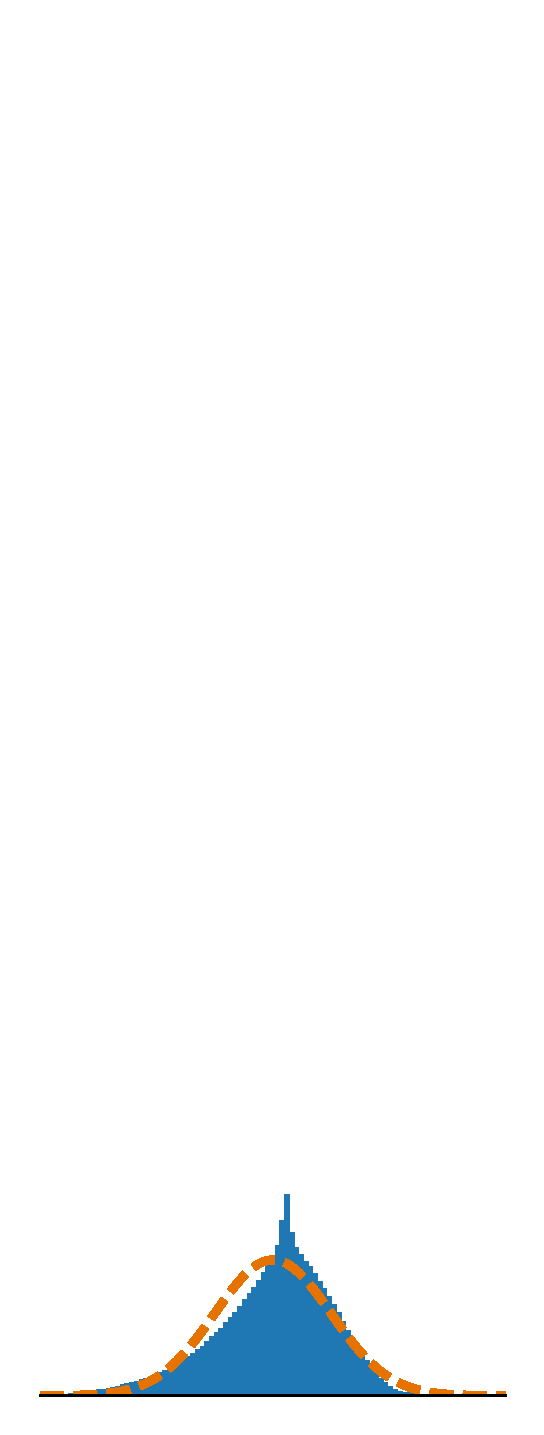
\includegraphics[width=0.33\linewidth,trim={0 0 0 20cm},clip]{BirdVox-pcen_EoverMplusEps_histogram.eps}}
% \\
% \subfloat[Renormalization with soft threshold and exponent: $\mathbf{E} \mapsto \dfrac{\mathbf{E}}{(\varepsilon+(\mathbf{E}\ast\boldsymbol{\phi}))^\alpha}$.]{%
% 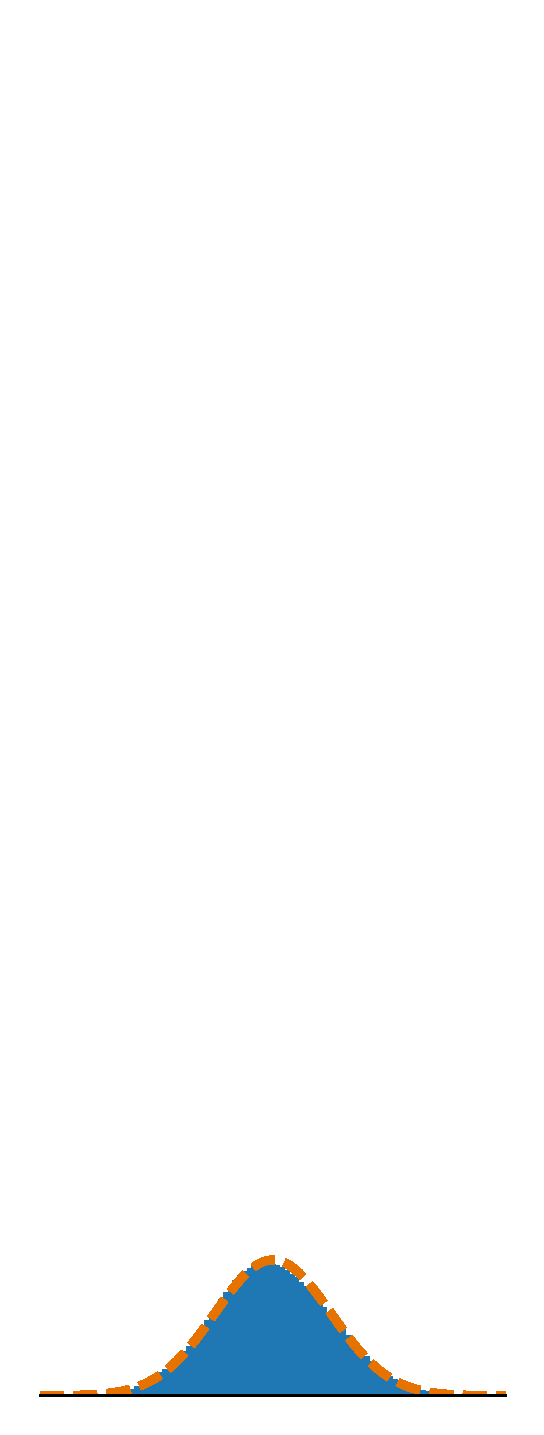
\includegraphics[width=0.33\linewidth,trim={0 0 0 20cm},clip]{SONYC-pcen_G_histogram.eps}
% 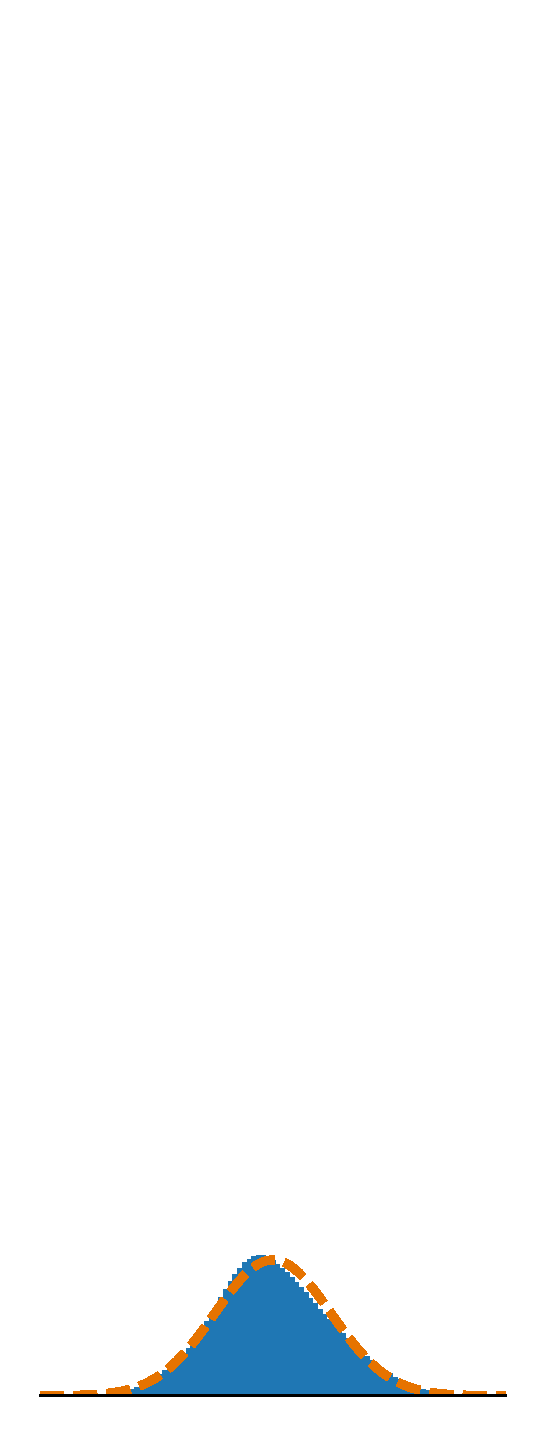
\includegraphics[width=0.33\linewidth,trim={0 0 0 20cm},clip]{DCASE2013-pcen_G_histogram.eps}
% 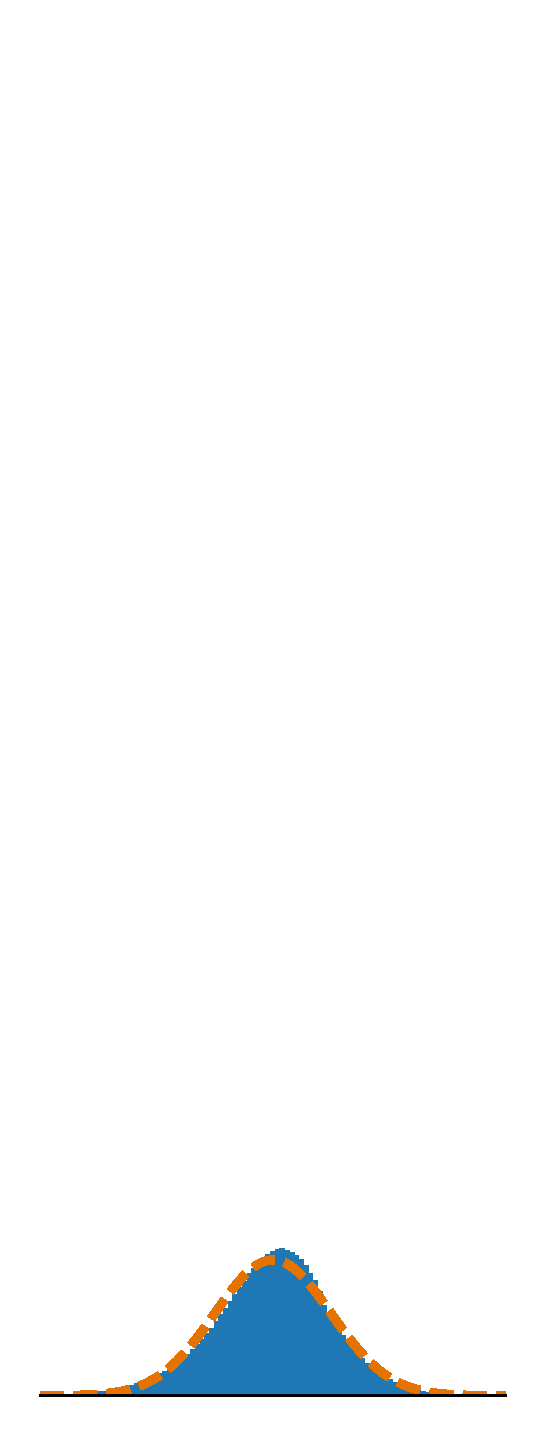
\includegraphics[width=0.33\linewidth,trim={0 0 0 20cm},clip]{BirdVox-pcen_G_histogram.eps}}
% \\
% \subfloat[Per-channel energy normalization (PCEN).]{%
% 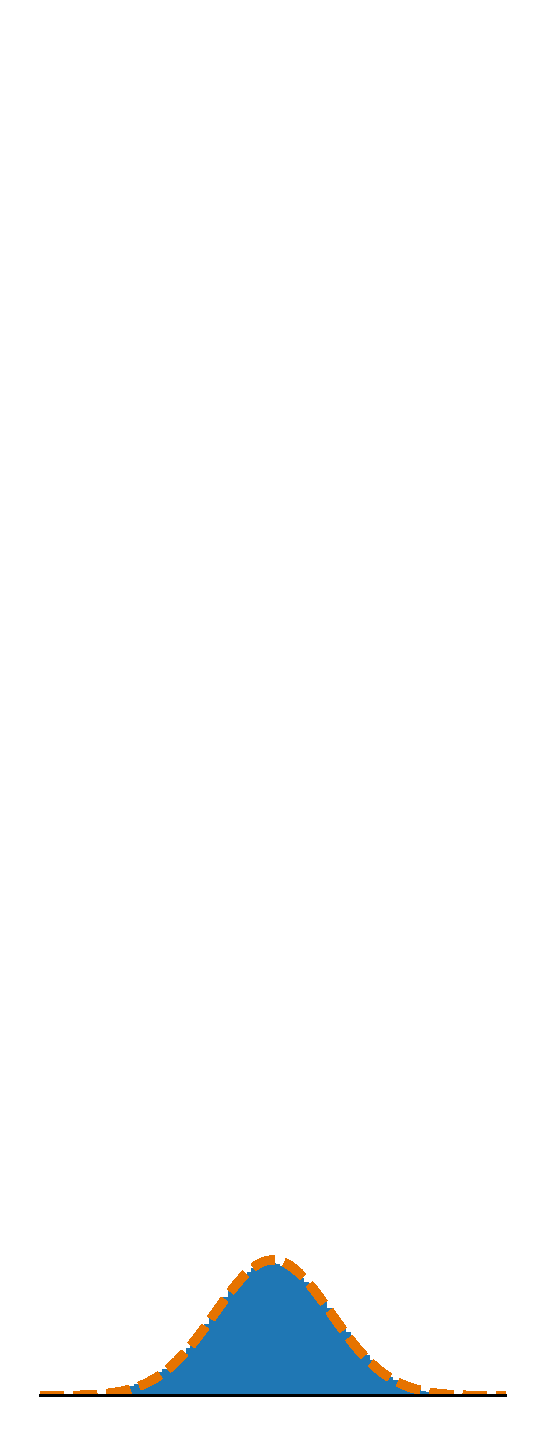
\includegraphics[width=0.33\linewidth,trim={0 0 0 21cm},clip]{SONYC-pcen_PCEN_histogram.eps}
% 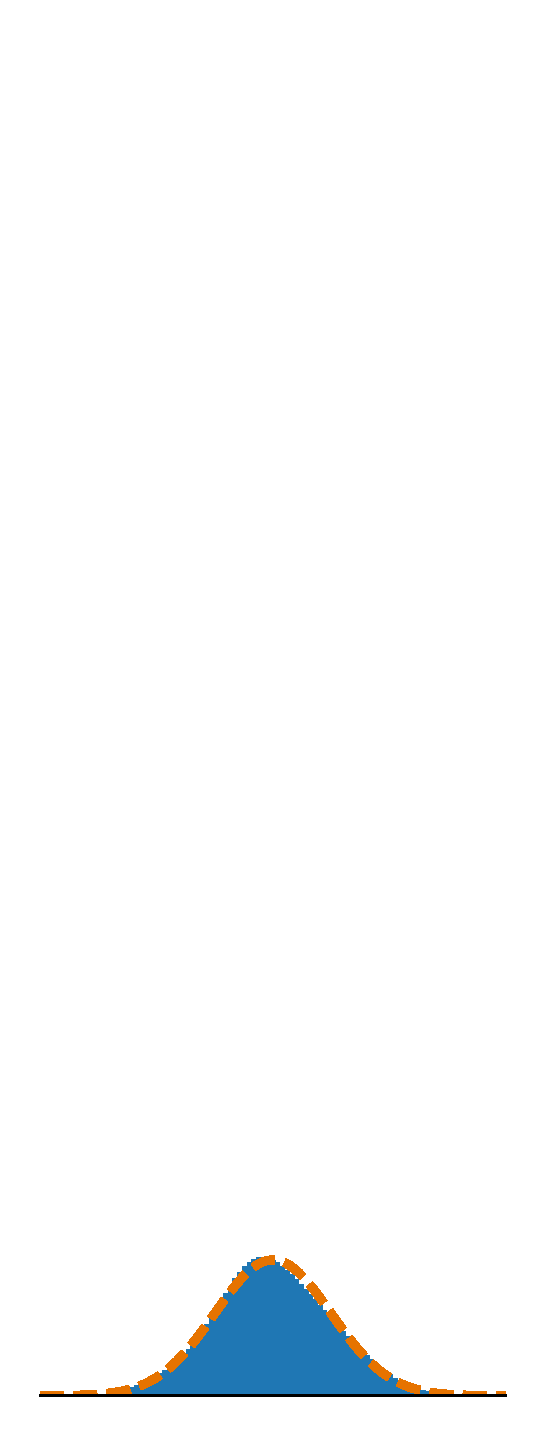
\includegraphics[width=0.33\linewidth,trim={0 0 0 21cm},clip]{DCASE2013-pcen_PCEN_histogram.eps}
% 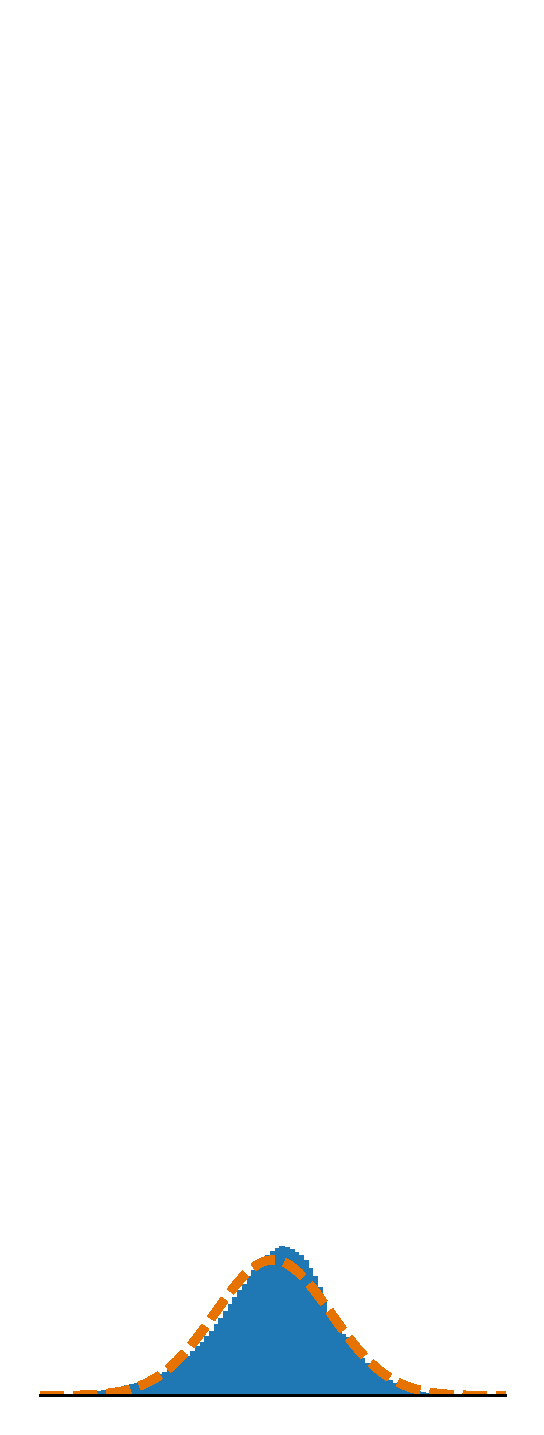
\includegraphics[width=0.33\linewidth,trim={0 0 0 21cm},clip]{BirdVox-pcen_PCEN_histogram.eps}}
% \caption{Distributions of magnitudes in the mel-frequency spectrogram after logmelspec (a),  and PCEN (c), as estimated on three datasets of acoustic scenes:
% SONYC (left); DCASE 2013 (middle); and BirdVox (right).
% Each distribution is scaled to null mean and unit variance, and discretized with $500$ histogram bins ranging between $-4$ and $4$.
% For comparison, the dashed line indicates the standard normal distribution.
% See Subsection \ref{sub:gaussianization} for details.}
% \label{fig:gaussianization-extended}
% \end{figure}

% \begin{figure}
% \centering
% \subfloat[Logarithmic transformation.]{
% \stackunder{SONYC}{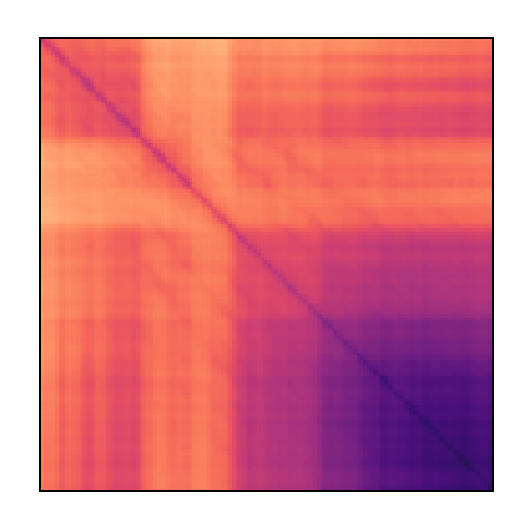
\includegraphics[width=0.33\linewidth]{SONYC-pcen_logE_covariance.eps}}
% \stackunder{DCASE 2013}{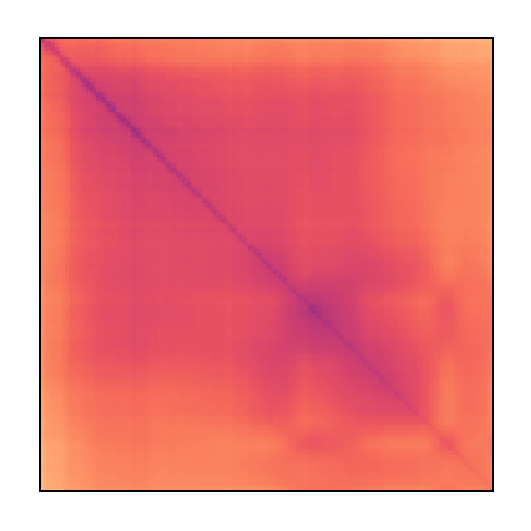
\includegraphics[width=0.33\linewidth]{DCASE2013-pcen_logE_covariance.eps}}
% \stackunder{BirdVox}{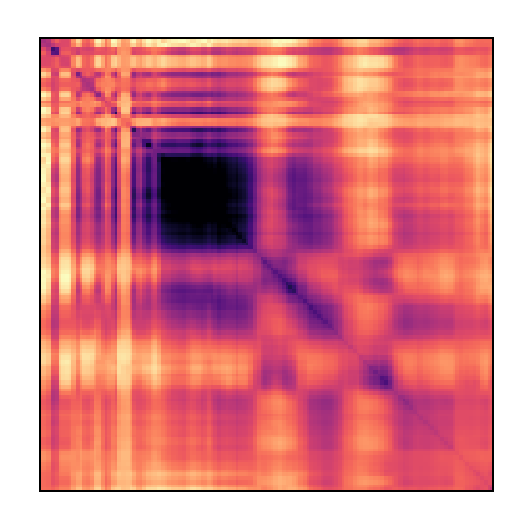
\includegraphics[width=0.33\linewidth]{BirdVox-pcen_logE_covariance.eps}}}
% \\
% \subfloat[Simple renormalization.]{
% \stackunder{SONYC}{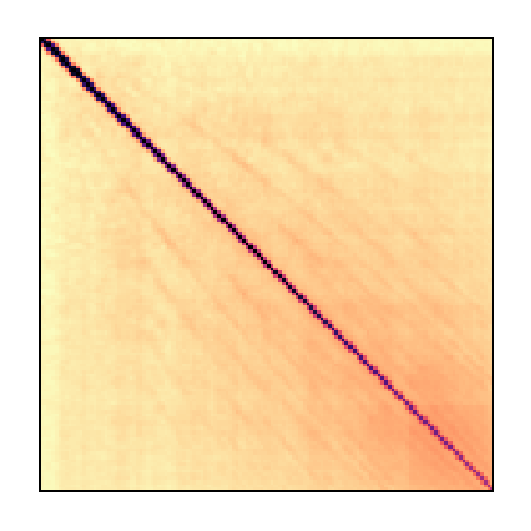
\includegraphics[width=0.33\linewidth]{SONYC-pcen_EoverM_covariance.eps}}
% \stackunder{DCASE 2013}{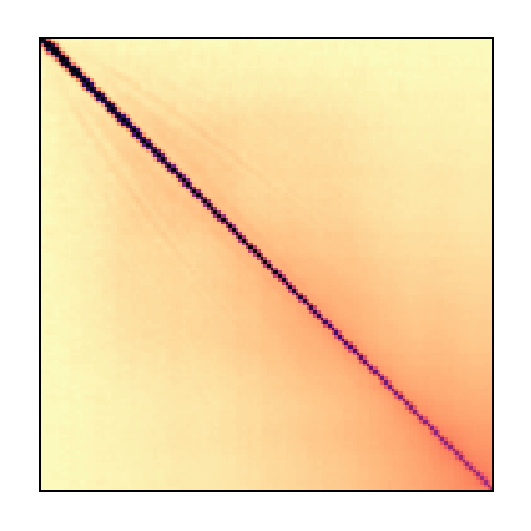
\includegraphics[width=0.33\linewidth]{DCASE2013-pcen_EoverM_covariance.eps}}
% \stackunder{BirdVox}{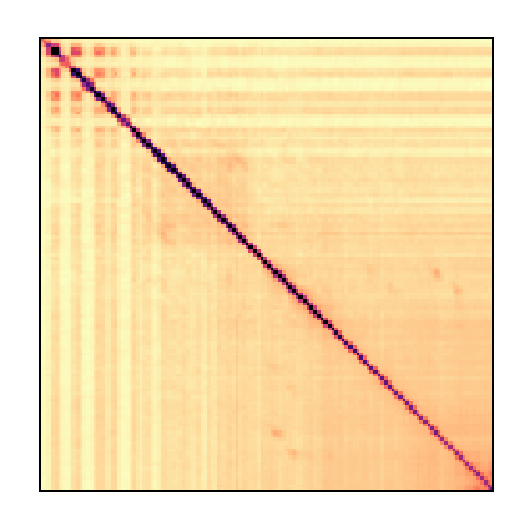
\includegraphics[width=0.33\linewidth]{BirdVox-pcen_EoverM_covariance.eps}}}
% \\
% \subfloat[Simple renormalization.]{
% \stackunder{SONYC}{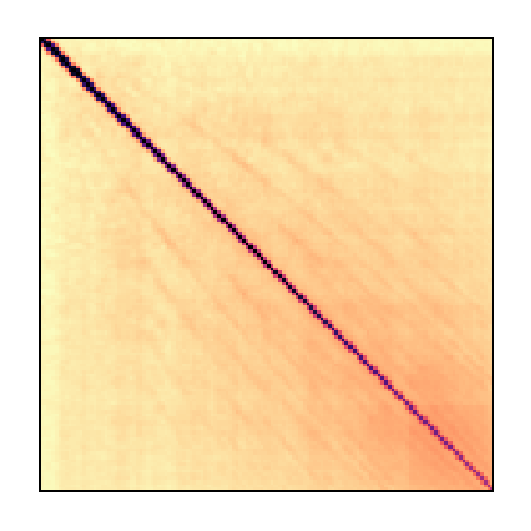
\includegraphics[width=0.33\linewidth]{SONYC-pcen_EoverMplusEps_covariance.eps}}
% \stackunder{DCASE 2013}{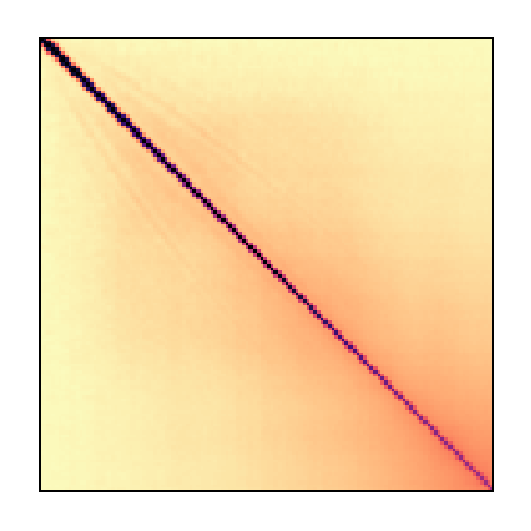
\includegraphics[width=0.33\linewidth]{DCASE2013-pcen_EoverMplusEps_covariance.eps}}
% \stackunder{BirdVox}{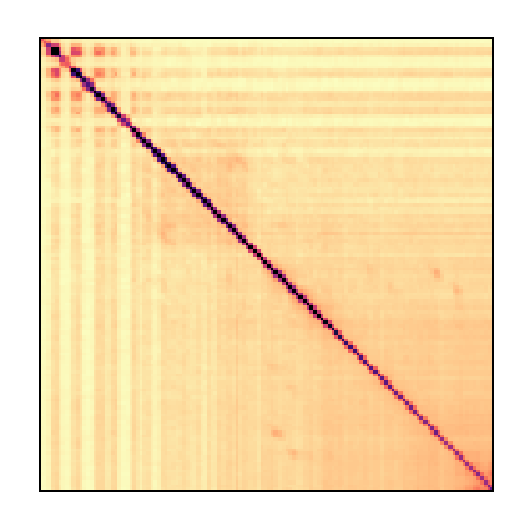
\includegraphics[width=0.33\linewidth]{BirdVox-pcen_EoverMplusEps_covariance.eps}}}
% \\
% \subfloat[Renormalization with soft threshold and exponent.]{
% \stackunder{SONYC}{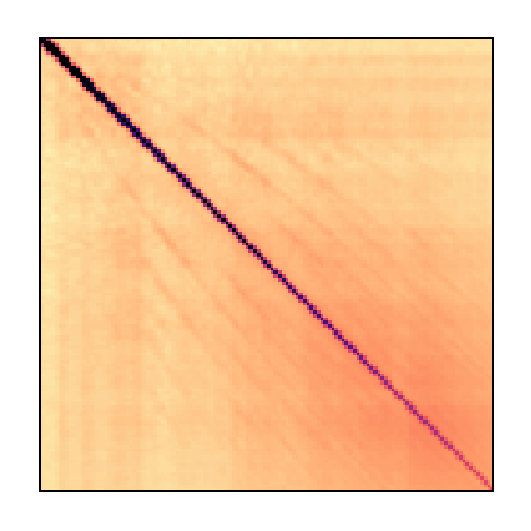
\includegraphics[width=0.33\linewidth]{SONYC-pcen_G_covariance.eps}}
% \stackunder{DCASE 2013}{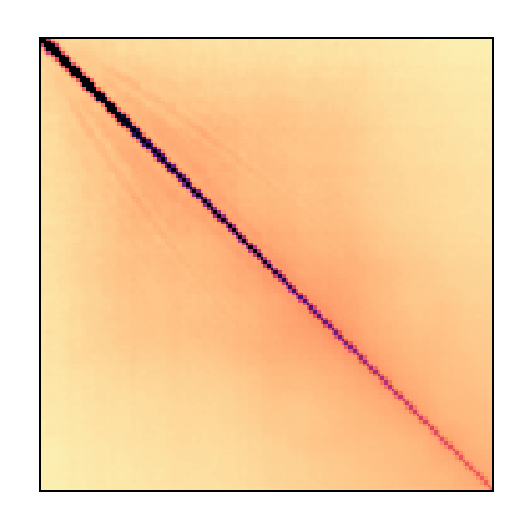
\includegraphics[width=0.33\linewidth]{DCASE2013-pcen_G_covariance.eps}}
% \stackunder{BirdVox}{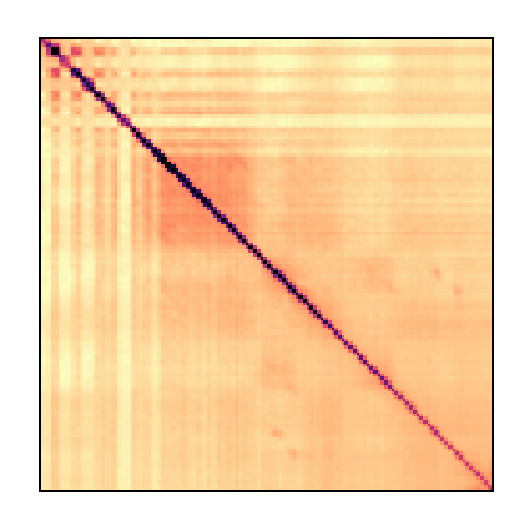
\includegraphics[width=0.33\linewidth]{BirdVox-pcen_G_covariance.eps}}}
% \\
% \subfloat[Per-channel energy normalization (PCEN).]{
% 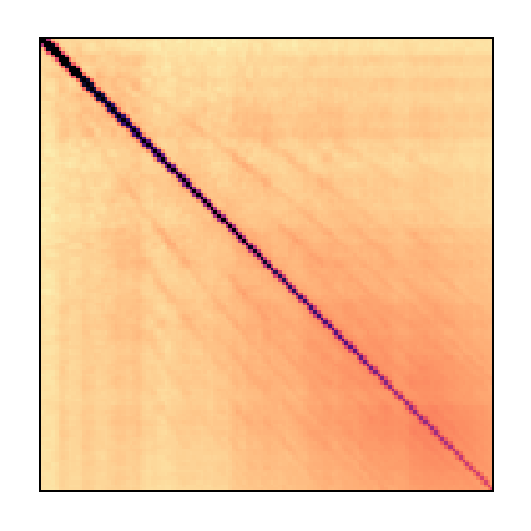
\includegraphics[width=0.33\linewidth]{SONYC-pcen_PCEN_covariance.eps}
% 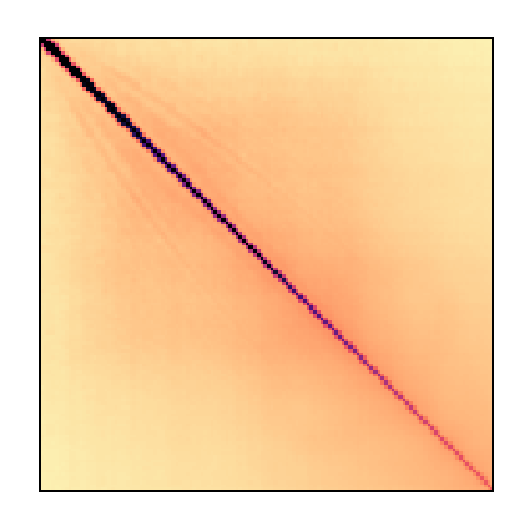
\includegraphics[width=0.33\linewidth]{DCASE2013-pcen_PCEN_covariance.eps}
% 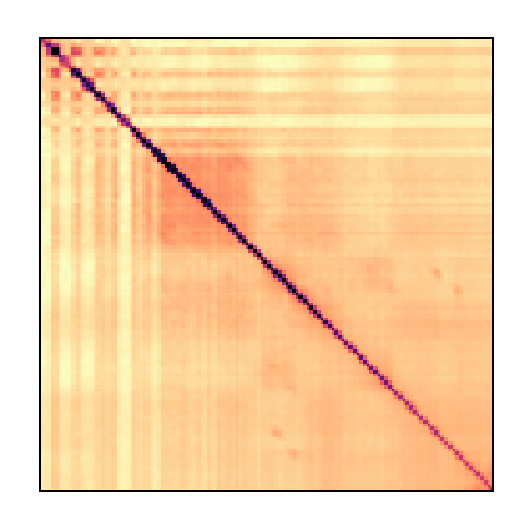
\includegraphics[width=0.33\linewidth]{BirdVox-pcen_PCEN_covariance.eps}}
% \caption{Covariance matrices of frequency channels after logarithmic transformation (a) and PCEN (b), as estimated on three datasets of acoustic scenes: SONYC (left); DCASE 2013 (middle); and BirdVox (right).
% Darker shades indicate larger covariances in absolute value. See Subsection \ref{sub:decorrelation} for details.}
% \label{fig:decorrelation-extended}
% \end{figure}

\subsection{Proof of Proposition \ref{prop:temporal-integration} on temporal integration}

% \begin{prop*}
% Let $0 < s < 1$ and $\tau >0$.
% The infinite impulse reponse filter $\boldsymbol{\phi}_T$ defined by the autoregressive process
% \begin{equation}
% \mathbf{y}(t) = (\mathbf{x} \ast \boldsymbol{\phi}_T)(t) = s \mathbf{x}(t) + (1-s) \mathbf{y}(t - \tau),
% \end{equation}
% has a gain $\SI{0}{\decibel}$ at \SI{0}{\hertz}, a cutoff frequency
% \begin{equation}
% \omega_\mathrm{c} = \arccos\left(1 - \frac{s^2}{2 (1-s)}\right)
% \end{equation}
% at \SI{3}{\decibel}, and a sidelobe falloff of \SI{10}{\decibel} per decade near $\omega_\mathrm{c}$.
% \end{prop*}

\begin{proof}
At a discrete rate $\tau^{-1}$, the Fourier transform of $\boldsymbol{\phi}_T$ is
\begin{align}
\widehat{\boldsymbol{\phi}_T}  (\omega) =
\mathcal{Z}\{\boldsymbol{\phi}_T\}(\mathrm{e}^{\mathrm{j}\omega})
= \dfrac{s \mathrm{e}^{\mathrm{j}\omega}}{\mathrm{e}^{\mathrm{j}\omega} - (1-s)}.
\end{align}
The squared magnitude of the denominator simplifies as
\begin{align}
\vert \mathrm{e}^{\mathrm{j}\omega} - (1-s) \vert^2
& = (\cos \omega - (1-s))^2 + (\sin \omega)^2 \nonumber \\
& = 1 + (1-s)^2 - 2 (1-s) \cos \omega \nonumber \\
& = (1 - (1-s))^2 + 2 (1-s) (1 - \cos \omega) \nonumber \\
& = s^2 + 2 (1-s) (1 - \cos \omega).
\end{align}
Let $\omega_0 = \frac{s}{\sqrt{1-s}}$.
The equivalent $(1 - \cos \omega) \sim \frac{\omega^2}{2}$ at the limit $\omega \rightarrow 0$ indicates a quadratic decay in the lowest frequencies, \ie{} a sidelobe falloff of $\SI{10}{\decibel}$ per decade.
On one hand, the double inequality $-1 \leq \cos \omega \leq 1$ leads to 
\begin{equation}
\dfrac{\omega_0^2}{\omega_0^2 + 2} \leq \vert \widehat{\boldsymbol{\phi}_T} \vert^2 (\omega) \leq 1.
\end{equation}
The upper (\resp{} lower) bound is attained if and only if $\omega = 0$ (\resp{} $\omega = \pi$).
Consequently, $\boldsymbol{\phi}_T$ has a DC gain of $\SI{0}{\decibel}$ at $\SI{0}{\Hz}$, and a gain of $10 \log_{10} \frac{\omega_0^2}{2+\omega_0^2}$ (in dB) at the Nyquist frequency.
On the other hand, the cutoff frequency at $\SI{3}{\decibel}$ $\omega_{\mathrm{c}}$ is defined by $\vert\widehat{\boldsymbol{\phi}_T}\vert^2(\omega_c) = \frac{1}{2}$, which can be reformulated as
\begin{equation}
1 - \cos \omega_\mathrm{c} = \frac{ s^2}{2(1-s)} = \frac{\omega_0^2}{2}.
\label{eq:cutoff-frequency}
\end{equation}
Solving Equation \ref{eq:cutoff-frequency} with $\omega_\mathrm{c} > 0$ completes the proof.
\end{proof}

\begin{remark}
For large $T$, we can approximate $\omega_{c}$ by $\omega_0$, which is polynomial in $s$.
Indeed, applying Taylor's theorem to the cosine function yields the inequality $\vert 1 - \cos \omega - \frac{\omega^2}{2}\vert \leq \frac{\omega^4}{24}$, of which we deduce
\begin{equation}
\omega_0 \leq \omega_\mathrm{c} \leq \dfrac{\omega_0}{\sqrt{1 - \dfrac{\omega_\mathrm{c}^2}{12}}}
%\leq 6 \left(1-\sqrt{1-\dfrac{\omega_0}{3}}\right)
\leq \omega_0 + \dfrac{\omega_0^2}{12} + \dfrac{\omega_0^3}{12}.
\end{equation}
\end{remark}


\subsection{Proof of Proposition \ref{prop:gain-control} on adaptive gain control}

% \begin{prop*}
% Let $0 < \alpha < 1$ and $\varepsilon > 0$.
% The adaptive gain level
% \begin{equation}
% \mathbf{G} = \dfrac{ \mathbf{E} }{ (\mathbf{M}+\varepsilon)^\alpha}
% \end{equation}
% is asymptotically equivalent to:
% \begin{enumerate}[label=(\roman*)]
% \item $\mathbf{E}(t,f) / \varepsilon^\alpha$ if $\mathbf{M}(t,f) \ll \varepsilon$, and to
% \item $\mathbf{E}(t,f) / \mathbf{M}(t,f)^\alpha$ if $\mathbf{M}(t,f) \gg \varepsilon$.
% \end{enumerate}
% \end{prop*}

\begin{proof}
First, applying Taylor's theorem to $x \mapsto (1+x)^{-\alpha}$ gives $\left \vert (\mathbf{M} + \varepsilon)^{-\alpha} - \varepsilon^{-\alpha} \right \vert \leq \alpha \frac{\mathbf{M}}{\varepsilon^{1+\alpha}}$, from which we deduce (i) with a relative error of at most $\alpha \frac{\mathbf{M}}{\varepsilon}$.
Symmetrically, we have $\left \vert (\mathbf{M} + \varepsilon)^{-\alpha} - \mathbf{M}^{-\alpha} \right \vert \leq \alpha \frac{\varepsilon}{\mathbf{M}^{1+\alpha}}$ from which we deduce (ii) with a relative error of at most $\alpha \frac{\varepsilon}{\mathbf{M}}$.
\end{proof}



\subsection{Proof of Proposition \ref{prop:loudness-compression} on dynamic range compression}

% \begin{prop*}
% Let $0 < r < 1$ and $\delta > 0$.
% The per-channel energy normalization 
% \begin{equation}
% \mathbf{PCEN} = (\mathbf{G} + \delta)^r - \delta^r
% \end{equation}
% is asymptotically equivalent to:
% \begin{enumerate}[label=(\roman*)]
% \item $r \delta^{(r-1)} \mathbf{G}$ if $\mathbf{G} \ll \delta$, and to
% \item $\mathbf{G}^r$ if $\mathbf{G} \gg \delta$.
% \end{enumerate}
% \end{prop*}

\begin{proof}
First, applying Taylor's theorem to $x \mapsto (1+x)^r$ gives
$\vert \mathbf{PCEN} - r \delta^{(r-1)} \mathbf{G} \vert \leq \frac{1-r}{2} r \delta^{(r-1)} \mathbf{G}^2$, of which we deduce (i) with a relative error of at most $\frac{1-r}{2} \mathbf{G}$.
Secondly, we have
$\left \vert \left(1 + \frac{1}{\mathbf{G}^r}\right)^r - \left(r + \frac{r}{\mathbf{G}^r} \right)\right \vert \leq \frac{r(1-r)}{2\mathbf{G}^{2r}}$, which, after adding the constant $(1-r)$, leads to (ii) with a relative error of at most $\frac{1-r}{\mathbf{G}^r} (1+\frac{r}{2\mathbf{G}^r})$ by application of the triangular inequality.
\end{proof}

\begin{remark}
In both cases, the relative error is null if and only if $r=1$, \ie{} if there is no root compression.
\end{remark}


\subsection{Proof of Proposition \ref{prop:T-to-s} on the link between $T$ and $s$}

% \begin{prop*}
% Let $\tau > 0$ and $T>2\tau$.
% At the discrete rate $\tau^{-1}$, let $\boldsymbol{\phi}_T$ an infinite impulse response filter of time scale $T$, defined by the autoregressive process
% \begin{equation}
% \mathbf{y}(t) = (\mathbf{x} \ast \boldsymbol{\phi}_T)(t) = s \mathbf{x}(t) + (1-s) \mathbf{y}(t - \tau).
% \end{equation}
% The weight $s$ in the equation above is equal to
% \begin{equation}
% s = \sqrt{1 - \cos \dfrac{2\pi \tau}{T}} \left(\sqrt{3 - \cos \dfrac{2\pi \tau}{T}} - \sqrt{1 - \cos \dfrac{2\pi \tau}{T}} \right).
% \end{equation}
% \end{prop*}

\begin{proof}
Let $\omega_0^2 = 2 \left(1 - \cos \frac{2\pi \tau}{T}\right)$.
Proposition \ref{prop:temporal-integration} yields
$\omega_0^2 = \frac{s^2}{(1-s)}$, and thus the quadratic equation
$s^2 + \omega_0^2 s - \omega_0^2 = 0$.
Its discriminant is $\Delta = \omega_0^4 + 4 \times \omega_0^2 = \omega_0^2 (\omega_0^2 + 4) > 0$, and its two real-valued roots are
\begin{equation}
s = \frac{- \omega_0^2 \pm \omega_0 \sqrt{\omega_0^2 +4}}{2}
= \frac{\omega_0}{2} \left(\pm\sqrt{\omega_0^2 + 4} - \omega_0\right)
\end{equation}
We retain the positive root $s > 0$. Replacing $\omega_0$ by its definition in the above completes the proof.
\end{proof}


\subsection{Proof of Proposition \ref{prop:invariance} on invariance to impedance curve}

\begin{prop*}
Let $\mathbf{s}(t)$ a realization of AWGN with null mean and unit variance.
Let $\mathbf{a}(t) > 0$ a deterministic amplitude envelope $\mathbf{h}(t)$ a filter.
Let $\mathbf{E}_\mathbf{x}(t,f)$ the mel-frequency spectrogram associated to the source-filter model $\mathbf{x}(t) = \mathbf{a}(t) \times (\mathbf{s}\ast\mathbf{h})(t)$.
If
\begin{enumerate}
\item $\forall t_0,\; \dfrac{\mathrm{d}\log \mathbf{a}}{\mathrm{d}t} (t_0) \ll \dfrac{1}{T}$,
\item $\forall t_0,\; \int_{t_0}^{t_0+\tau} \mathbf{h}(t)\;\mathrm{d}t \ll \dfrac{1}{\tau}$, and
\item $\forall f_0,\; \dfrac{\mathrm{d}\log \vert \widehat{\mathbf{h}}\vert}{\mathrm{d}f}(f_0) \ll
%\dfrac{1}{\mathrm{mel}^{-1}\left(\mathrm{mel}(f_0) \pm \dfrac{\mathrm{mel}(f_{\max}) - \mathrm{mel}(f_{\min})}{N}\right)}
\dfrac{1}{\Delta f_0},
$
\end{enumerate}
where $\Delta f_0$ is the frequency interval between $f_0$ and its adjacent subbands on the mel scale,
then $\mathbf{PCEN_x}(t,f) \approx \mathbf{PCEN_s}(t,f)$.
\end{prop*}

\renewenvironment{proof}{\emph{Proof.}}{\qed}

\begin{proof}
We adapt a result from [25].
The mel-frequency spectrogram $\mathbf{E}_{\mathbf{x}}(t,f)$ can be defined as the complex modulus of the convolution between the signal $\mathbf{x}(t)$ and a filterbank $\mathbf{\psi}_{f} (t)$ of $N$ whose center frequencies $f$ are tuned to the mel scale, ranging betweeen $f_{\min}$ and $f_{\max}$.
For a given $f$, the first hypothesis allows to factorize the amplitude envelope $\mathbf{a}(t)$ out of the convolution $(\mathbf{s}\ast\mathbf{h}\ast\boldsymbol{\psi}_f)(t)$
Furthermore, one has:
\begin{align}
\mathbf{E}_{(\mathbf{s}\ast\mathbf{h})} (t,f) & =
\vert \mathbf{s} \ast \mathbf{h} \ast \boldsymbol{\psi}_f \vert (t)
\nonumber \\
& = \dfrac{1}{2\pi} \left \vert \int_{\mathbb{R}} \widehat{\mathbf{s}}(\omega) \widehat{\mathbf{h}}(\omega) \widehat{\boldsymbol{\psi}_f}(\omega) \exp(2 \pi \mathrm{i} \omega t) \;\mathrm{d}t \right \vert.
\end{align}
The second and third hypotheses allow to approximate $\widehat{\mathbf{h}}(\omega)$ by $\widehat{\mathbf{h}}(f)$ in the equation above.
This approximation leads to $\mathbf{E}_{(\mathbf{s}\ast\mathbf{h})} (t,f) \approx \vert\widehat{\mathbf{h}}\vert (f) \mathbf{E}_{\mathbf{s}} (t,f)$.
Combining the factorization of the amplitude term $\mathbf{a}(t)$ with the factorization of the filter $\vert\mathbf{h}\vert(\omega)$ leads to an approximation of the form:
\begin{align}
\big\vert \mathbf{E}_\mathbf{x}(t,f) - \mathbf{a}(t) \vert\widehat{\mathbf{h}}\vert(f) \mathbf{E}_\mathbf{s}(t,f) \big\vert = \boldsymbol{\eta}(t,f).
\end{align}
An upper bound on the expectation of the stochastic residual $\boldsymbol{\eta}$ is given in [25, Appendix].
Likewise, the first hypothesis allows to approximate $\mathbf{M}_\mathbf{x}(t,f)$ by $\mathbf{a}(t) \vert \widehat{\mathbf{h}}(f) \vert \mathbf{M}_s(t,f)$ with a stochastic residual term $\mathbf{\nu}(t,f)$ of bounded expectation.
In the active regime ($\mathbf{M}\gg\varepsilon$), AGC cancels $\mathbf{a}(t)$ and $\vert\widehat{h}(f)\vert$ in Equation \ref{eq:gain-control}.
Thus, Proposition \ref{prop:gain-control} leads to the inequality
\begin{equation}
\vert \mathbf{G}_\mathrm{x} - \mathbf{G}_{\mathrm{s}} \vert (t,f)\leq
\dfrac{\boldsymbol{\eta}(t,f)}{(\varepsilon + \mathbf{M}_{\mathbf{s}}(t,f))^\alpha} + \dfrac{\alpha \boldsymbol{\nu}(t,f)}{(\varepsilon+\mathbf{M}_\mathbf{s} (t,f))^{1+\alpha}}.
\label{eq:G-approx}
\end{equation}
Because $\delta > 1$ and $r \leq 1$, DRC is nonexpansive (see Proposition \ref{prop:loudness-compression}).
Therefore, it maps each member of the approximate equality $\mathbf{G}_\mathbf{x} (t,f) \approx \mathbf{G}_\mathbf{s}(t,f)$ to $\mathbf{PCEN}_\mathbf{x} (t,f) \approx \mathbf{PCEN}_\mathbf{s}(t,f)$ while reducing the expectation of the residual (right-hand side of Equation \ref{eq:G-approx}), which completes the proof.
\end{proof}

% Can use something like this to put references on a page
% by themselves when using endfloat and the captionsoff option.
%\ifCLASSOPTIONcaptionsoff
%  \newpage
%\fi
%\newpage


% trigger a \newpage just before the given reference
% number - used to balance the columns on the last page
% adjust value as needed - may need to be readjusted if
% the document is modified later
%-\IEEEtriggeratref{8}
% The "triggered" command can be changed if desired:
%\IEEEtriggercmd{\enlargethispage{-5in}}

% references section

% can use a bibliography generated by BibTeX as a .bbl file
% BibTeX documentation can be easily obtained at:
% http://mirror.ctan.org/biblio/bibtex/contrib/doc/
% The IEEEtran BibTeX style support page is at:
% http://www.michaelshell.org/tex/ieeetran/bibtex/
%\bibliographystyle{IEEEtran}
% argument is your BibTeX string definitions and bibliography database(s)
%\bibliography{IEEEabrv,lostanlen2018spl}
%
% <OR> manually copy in the resultant .bbl file
% set second argument of \begin to the number of references
% (used to reserve space for the reference number labels box)
%\begin{thebibliography}{1}

%\bibitem{IEEEhowto:kopka}
%H.~Kopka and P.~W. Daly, \emph{A Guide to \LaTeX}, 3rd~ed.\hskip 1em plus
%  0.5em minus 0.4em\relax Harlow, England: Addison-Wesley, 1999.

%\end{thebibliography}

% biography section
% 
% If you have an EPS/PDF photo (graphicx package needed) extra braces are
% needed around the contents of the optional argument to biography to prevent
% the LaTeX parser from getting confused when it sees the complicated
% \includegraphics command within an optional argument. (You could create
% your own custom macro containing the \includegraphics command to make things
% simpler here.)
%\begin{IEEEbiography}[{\includegraphics[width=1in,height=1.25in,clip,keepaspectratio]{mshell}}]{Michael Shell}
% or if you just want to reserve a space for a photo:

%\begin{IEEEbiography}{Michael Shell}
%Biography text here.
%\end{IEEEbiography}

% if you will not have a photo at all:
%\begin{IEEEbiographynophoto}{John Doe}
%Biography text here.
%\end{IEEEbiographynophoto}

% insert where needed to balance the two columns on the last page with
% biographies
%\newpage

%\begin{IEEEbiographynophoto}{Jane Doe}
%Biography text here.
%\end{IEEEbiographynophoto}

% You can push biographies down or up by placing
% a \vfill before or after them. The appropriate
% use of \vfill depends on what kind of text is
% on the last page and whether or not the columns
% are being equalized.

%\vfill

% Can be used to pull up biographies so that the bottom of the last one
% is flush with the other column.
%\enlargethispage{-5in}


% that's all folks
\end{document}


% An example of a floating figure using the graphicx package.
% Note that \label must occur AFTER (or within) \caption.
% For figures, \caption should occur after the \includegraphics.
% Note that IEEEtran v1.7 and later has special internal code that
% is designed to preserve the operation of \label within \caption
% even when the captionsoff option is in effect. However, because
% of issues like this, it may be the safest practice to put all your
% \label just after \caption rather than within \caption{}.
%
% Reminder: the "draftcls" or "draftclsnofoot", not "draft", class
% option should be used if it is desired that the figures are to be
% displayed while in draft mode.
%
%\begin{figure}[!t]
%\centering
%\includegraphics[width=2.5in]{myfigure}
% where an .eps filename suffix will be assumed under latex, 
% and a .pdf suffix will be assumed for pdflatex; or what has been declared
% via \DeclareGraphicsExtensions.
%\caption{Simulation results for the network.}
%\label{fig_sim}
%\end{figure}

% Note that the IEEE typically puts floats only at the top, even when this
% results in a large percentage of a column being occupied by floats.


% An example of a double column floating figure using two subfigures.
% (The subfig.sty package must be loaded for this to work.)
% The subfigure \label commands are set within each subfloat command,
% and the \label for the overall figure must come after \caption.
% \hfil is used as a separator to get equal spacing.
% Watch out that the combined width of all the subfigures on a 
% line do not exceed the text width or a line break will occur.
%

%
% Note that often IEEE papers with subfigures do not employ subfigure
% captions (using the optional argument to \subfloat[]), but instead will
% reference/describe all of them (a), (b), etc., within the main caption.
% Be aware that for subfig.sty to generate the (a), (b), etc., subfigure
% labels, the optional argument to \subfloat must be present. If a
% subcaption is not desired, just leave its contents blank,
% e.g., \subfloat[].


% An example of a floating table. Note that, for IEEE style tables, the
% \caption command should come BEFORE the table and, given that table
% captions serve much like titles, are usually capitalized except for words
% such as a, an, and, as, at, but, by, for, in, nor, of, on, or, the, to
% and up, which are usually not capitalized unless they are the first or
% last word of the caption. Table text will default to \footnotesize as
% the IEEE normally uses this smaller font for tables.
% The \label must come after \caption as always.
%
%\begin{table}[!t]
%% increase table row spacing, adjust to taste
%\renewcommand{\arraystretch}{1.3}
% if using array.sty, it might be a good idea to tweak the value of
% \extrarowheight as needed to properly center the text within the cells
%\caption{An Example of a Table}
%\label{table_example}
%\centering
%% Some packages, such as MDW tools, offer better commands for making tables
%% than the plain LaTeX2e tabular which is used here.
%\begin{tabular}{|c||c|}
%\hline
%One & Two\\
%\hline
%Three & Four\\
%\hline
%\end{tabular}
%\end{table}


% Note that the IEEE does not put floats in the very first column
% - or typically anywhere on the first page for that matter. Also,
% in-text middle ("here") positioning is typically not used, but it
% is allowed and encouraged for Computer Society conferences (but
% not Computer Society journals). Most IEEE journals/conferences use
% top floats exclusively. 
% Note that, LaTeX2e, unlike IEEE journals/conferences, places
% footnotes above bottom floats. This can be corrected via the
% \fnbelowfloat command of the stfloats package.